\documentclass[11pt, letterpaper]{article}
\usepackage[utf8]{inputenc}
\usepackage[letterpaper, margin=0.5in]{geometry}
\usepackage{amsmath}
\usepackage{amssymb}
\usepackage{amsthm}
\usepackage{graphicx}
\usepackage{listings}
\usepackage[font=scriptsize]{caption}
\usepackage{subcaption}
\usepackage{xcolor}
\graphicspath{ {.} }
\captionsetup{justification=raggedright, singlelinecheck=false}

\author{Ryan Tang}
\title{STA 602 HW 9}
\date{November 4th 2022}

\begin{document}
\maketitle

\section{Exercise 7.1}
\paragraph{(a) Jeffrey Prior on the Joint Parameters}
The Jeffrey prior is $p_J(\theta, \Sigma) \propto |\Sigma|^{-(p+2)/2}$. It is not a proper probability density function because it doesn't integrate to 1 and doesn't ensure $\Sigma$ to be positive definite, and symmetric. The only possible way is when the Inverse-Wishart distribution's $\nu_o > p - 1$, where $p$ is the dimension of $X \in \mathbb{R}^p$ in our observations. But the Jeffrey prior implies $\nu_o = 0$, which doesn't guarantee a proper $\Sigma$. Well, we can use it as long as the sample size exceeds the $p-1$ threshold.

\paragraph{(b) Full conditionals}
\begin{align*}
    Y_i &\mathop{\thicksim}^{iid} \mathcal{N}(\theta, \Sigma) && Y_i \in \mathbb{R}^p \\
    p(Y|\theta, \Sigma) &=
        (2\pi)^{-pN/2} |\Sigma|^{-N/2} 
        \exp \left[ -\frac{1}{2} \sum_i^N (y_i-\theta)^{\intercal} \Sigma^{-1} (y_i-\theta) \right] \\
    p_J(\theta, \Sigma) &\propto |\Sigma|^{-(p+2)/2} \\
    p_J(\theta, \Sigma|Y) &\propto p_J(\theta, \Sigma) p(Y|\theta, \Sigma) \\
        &\propto |\Sigma|^{-N/2} |\Sigma|^{-(p+2)/2}
            \exp \left[ -\frac{1}{2} \sum_i^N (y_i-\theta)^{\intercal} \Sigma^{-1} (y_i-\theta) \right] \\
        &\propto |\Sigma|^{-(N+p+2)/2} 
            \exp \left[ -\frac{1}{2} \sum_i^N (y_i-\theta)^{\intercal} \Sigma^{-1} (y_i-\theta) \right] \\ \\
    p_J(\theta|Y, \Sigma) &\propto \exp \left[
            -\frac{1}{2} (\theta^{\intercal}(N\Sigma^{-1})\theta
            + \theta^{\intercal}(N\Sigma^{-1} \bar{y}))
        \right] \\
        &\thicksim \mathcal{N}(\theta|(N\Sigma^{-1})^{-1}N\Sigma^{-1} \bar{Y}, N\Sigma^{-1}) \\ \\
    p_J(\Sigma|Y, \theta) &\propto |\Sigma|^{-(N+p+2)/2} 
            \exp \left[ -\frac{1}{2} \sum_i^N (y_i-\theta)^{\intercal} \Sigma^{-1} (y_i-\theta) \right] \\
        &\propto |\Sigma|^{-(N+1+p+1)/2} \exp \left[ -\frac{1}{2} tr(S \Sigma^{-1}) \right] \\
        &\thicksim \text{inverse-Wishart}(\Sigma | N+1, S) \\
    S &= \sum_i^N (y_i - \theta)^{\intercal} (y_i - \theta)
\end{align*}

\newpage
\section{Exercise 7.2}
\paragraph{(a) Multivariate Normal MLE \& Unit Information Priors}
Here we show that the joint unit information priors consist of two proper conjugate priors for the multivariate Gaussian model. The parameterization of the two priors is just the mean $\bar{y}$ and the unit scatter matrix $\frac{1}{N}S_{\bar{y}}=\frac{1}{N}\sum_i^N(y_i-\bar{y})(y_i-\bar{y})^{\intercal}$ from MLE.
\begin{align*}
    \Lambda &= \Sigma^{-1} \\
    p(X|\theta, \Sigma) &= (2\pi)^{-pN/2} |\Lambda|^{N/2} 
        \exp \left[ -\frac{1}{2} \sum_i^N (y_i-\theta)^{\intercal} \Lambda (y_i-\theta) \right] \\
    \ell(\theta, \Sigma) &= \frac{N}{2} \log |\Lambda| -\frac{1}{2} \sum_i^N (y_i-\theta)^{\intercal} \Lambda (y_i-\theta) \\
    p_U(\theta, \Lambda) &\propto \exp[\frac{1}{N} \ell(\theta, \Lambda)] \\
        &\propto \exp \left[
            \frac{1}{2} \log |\Lambda| -\frac{1}{2N}
            \sum_i^N (y_i-\theta)^{\intercal} \Lambda (y_i-\theta)
        \right] \\
        &\propto |\Lambda|^{\frac{1}{2}} \exp \left[
            -\frac{1}{2N}
            \sum_i^N (y_i-\bar{y}+\bar{y}+\theta)^{\intercal} \Lambda (y_i-\bar{y}+\bar{y}+\theta)
        \right] \\
        &\propto |\Lambda|^{\frac{1}{2}} \exp \left[
            -\frac{1}{2N}
            tr[
                (\sum_i^N(y_i-\bar{y})(y_i-\bar{y})^{\intercal}
                + \sum_i^N(\bar{y}-\theta)(\bar{y}-\theta)^{\intercal}
                + \sum_i^N(y_i-\bar{y})(\bar{y}-\theta)^{\intercal})
                \Lambda
            ]
        \right] \\
        & \quad\quad \sum_i^N(y_i-\bar{y})(\bar{y}-\theta)^{\intercal} = 0 \\
        &\propto |\Lambda|^{\frac{1}{2}} \exp \left[
            -\frac{1}{2}
            tr[
                (\frac{1}{N}\sum_i^N(y_i-\bar{y})(y_i-\bar{y})^{\intercal}
                + \frac{1}{N}\sum_i^N(\bar{y}-\theta)(\bar{y}-\theta)^{\intercal})
                \Lambda
            ]
        \right] \\
        &\propto |\Lambda|^{\frac{1}{2}} \exp \left[
            -\frac{1}{2}
            tr[
                \frac{1}{N}\sum_i^N(y_i-\bar{y})(y_i-\bar{y})^{\intercal} \Lambda
                + (\bar{y}-\theta)(\bar{y}-\theta)^{\intercal} \Lambda
            ]
        \right] \\
        &\propto |\Lambda|^{\frac{1}{2}} \exp \left[
            -\frac{1}{2} tr[\frac{1}{N}S_{\bar{y}}\Lambda] - \frac{1}{2}(\bar{y}-\theta)^{\intercal} \Lambda (\bar{y}-\theta)
        \right] \\
        & \quad\quad \frac{1}{N}S_{\bar{y}} = \frac{1}{N}\sum_i^N(y_i-\bar{y})(y_i-\bar{y})^{\intercal} \\
        &\propto
            |\Lambda|^{\frac{p+1-p-1}{2}} \exp \left[ -\frac{1}{2} tr[\frac{1}{N}S_{\bar{y}}\Lambda] \right]
            |\Lambda|^{\frac{1}{2}} \exp \left[ - \frac{1}{2}(\bar{y}-\theta)^{\intercal} \Lambda (\bar{y}-\theta) \right] \\
        &= Wi(\Lambda|p+1, \frac{1}{N}S_{\bar{y}}) \mathcal{N}(\theta|\bar{y}, \Lambda^{-1}) \\
        &= p(\theta|\Lambda) p(\Lambda) \\ \\
    \theta|\Lambda &\thicksim \mathcal{N}(\bar{y}, \Lambda^{-1}) \\
    \Lambda &\thicksim Wi(p+1, \frac{1}{N}S_{\bar{y}}) \\
\end{align*}

\paragraph{(b) Unit Information Posterior}
If we use MLE's unit information priors, the posterior with the same data happens to be the same form with the effective sample size increased with $N$.
\begin{align*}
    p_U(\theta,\Lambda|Y) &\propto p_U(\Lambda) p_U(\theta|\Lambda) p(Y|\theta, \Lambda) \\
        &\propto
            |\Lambda|^{\frac{p+1-p-1}{2}} \exp \left[ -\frac{1}{2} tr[\frac{1}{N}S_{\bar{y}}\Lambda] \right]
            |\Lambda|^{\frac{1}{2}} \exp \left[ - \frac{1}{2} [
                \theta^{\intercal}\Lambda\theta - \theta^{\intercal}\Lambda\bar{y}]
            \right] \\
            &\quad\,\, \cdot 
            |\Lambda|^{N/2} \exp \left[
                -\frac{1}{2} [tr(S_{\bar{y}}\Lambda) + \theta^{\intercal}N\Lambda\theta - \theta^{\intercal}N\Lambda\bar{y}]
            \right] \\
        &\propto 
            |\Lambda|^{\frac{N+p+1-p-1}{2}} \exp \left[ -\frac{1}{2} tr[\frac{N+1}{N}S_{\bar{y}}\Lambda] \right]
            |\Lambda|^{\frac{1}{2}} \exp \left[ - \frac{1}{2} [
                \theta^{\intercal}(\Lambda+N\Lambda)\theta - \theta^{\intercal}(\Lambda+N\Lambda)\bar{y}
            \right] \\
        &\propto Wi(N+p+1, \frac{N+1}{N}S_{\bar{y}}) \mathcal{N}((\Lambda+N\Lambda)^{-1}(\Lambda+N\Lambda)\bar{y}, (\Lambda+N\Lambda)^{-1})
\end{align*}


\section{Exercise 7.3}
\paragraph{(a) Posterior}
Since we have a known form in semi-conjugate, we can directly sample from it.
\begin{align*}
    \theta &\thicksim \mathcal{N}(\mu_o, \Sigma_o = \Lambda^{-1}) \\
    \theta|Y, \Sigma &\thicksim \mathcal{N}(
        \mu_n = \Sigma_n(\Lambda_o\mu_o+N\Lambda\bat{y}),
        \Sigma_n = (\Lambda_o + N\Lambda)^{-1}
    ) \\
    \Sigma &\thicksim IW(\nu_o, S_o) \\ 
    \Sigma|Y &\thicksim IW(v_o + n, (S_0+S_{\theta})^{-1} \\
    S_{\theta} &= \sum_i^N (y_i - \theta)(y_i - \theta)^{\intercal}
\end{align*}

\paragraph{(b) $\theta$ posteriors}
After the Bayesian updates, we can see Blue crabs generally have smaller body widths and rear widths than orange crabs.
\begin{figure*}[!h]
  \centering
  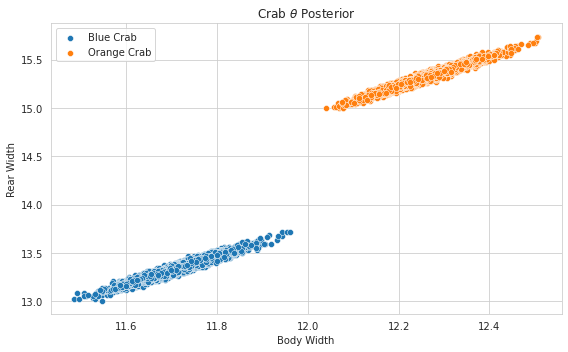
\includegraphics[width=1.0\textwidth]{3.1.png}
  \captionsetup{justification=centering}
  \caption{$\theta$ Posteriors Comparison of two Crabs}
\end{figure*}

\paragraph{(c) Correlation on $Sigma$ posteriors}
\begin{figure*}[!h]
  \centering
  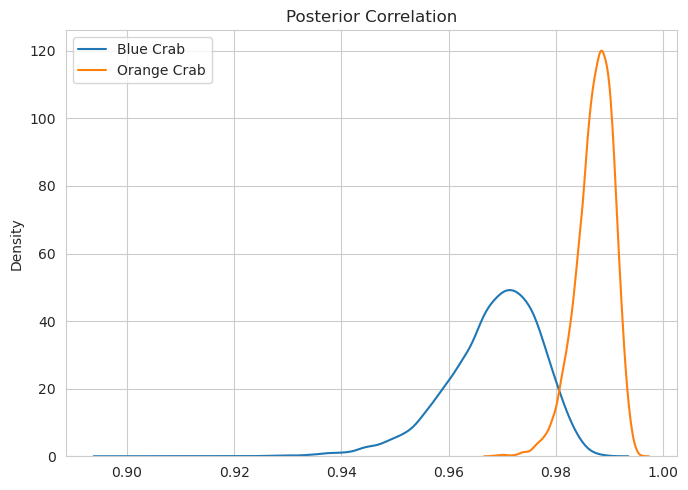
\includegraphics[width=0.6\textwidth]{3.2.png}
  \captionsetup{justification=centering}
  \caption{Correlation Posteriors Comparison of two Crabs. }
\end{figure*}

\end{document}